% !TEX program = xelatex
\documentclass[12pt,a4paper,fontset=none]{ctexart}

% === 中文字体：ctex fontset=none 必须手动定义全部六大字体族 ===
\setCJKmainfont{SimSun}
\setCJKsansfont{SimSun}
\setCJKmonofont{SimSun}
\setCJKfamilyfont{zhsong}{SimSun}
\setCJKfamilyfont{zhhei}{SimSun}
\setCJKfamilyfont{zhkai}{SimSun}
\setCJKfamilyfont{zhfs}{SimSun}
\setCJKfamilyfont{zhli}{SimSun}
\setCJKfamilyfont{zhyou}{SimSun}

% === 页面设置 ===
\usepackage[top=2.5cm,bottom=2.5cm,left=2.8cm,right=2.8cm]{geometry}
\usepackage{amsmath,amssymb,amsfonts}
\usepackage{mathtools}
\usepackage{booktabs}
\usepackage{graphicx}
\usepackage{float}
\usepackage{hyperref}
\usepackage{enumitem}
\usepackage{multirow}
\usepackage{array}
\usepackage{xcolor}

% === 自定义命令 ===
\newcommand{\R}{\mathbb{R}}
\newcommand{\st}{\text{s.t.}}
\newcommand{\code}[1]{\texttt{#1}}

% === 标题 ===
\title{\heiti\zihao{2} 高铁快运基地选址与规模多维协同优化\\案例分析报告}
\author{\kaishu\zihao{4} 胡鹏禹}
\date{\zihao{4} 2026年6月1日}

\begin{document}

\maketitle
\thispagestyle{empty}

\newpage
\tableofcontents
\newpage

% ============================================================
\section{问题理解}
% ============================================================

随着我国高速铁路网络的逐步成网与成熟运营，以"高时效、小批量、高附加值"为特征的高铁快运业务被广泛认为是铁路运输企业进军现代物流市场、实现商业化创收的战略性增长点。

在实际运输组织中，高铁快运主要涵盖三种模式：
\begin{itemize}
    \item \textbf{捎带模式}：利用既有载客动车组的二等座预留空间或确认列车空间，边际投资极小，不额外占用区间线路通过能力，但装载能力受限（客动捎带仅2.7吨/列，确认车8吨/列）；
    \item \textbf{货运动车组运输}：单列装载能力可达85吨，拥有极高的空间利用效率，但高度依赖具备存车、分拣、机械化装卸作业的专业快运物流基地；
    \item \textbf{中转作业}：在有基地的站点可以进行货物中转换装，中转成本为2.52元/吨次。
\end{itemize}

核心矛盾在于：如果基地建设数量过少或规模过小，虽然可以规避折旧风险，却无法有效吸纳货运动车组始发、终到和中转作业需求；反之，若基地过多过大，则会产生高额折旧和固定管理成本。因此，针对长周期运输需求预测数据，进行"轻重资产博弈"和"收益最大化"的运筹优化，是实现可持续商业化运营的核心挑战。

% ============================================================
\section{建模思路}
% ============================================================

我们设计并实施了"多阶段协同递进规划"的技术路线：

\begin{enumerate}[label=第\arabic*阶段：, leftmargin=*]
    \item \textbf{货流最短径路计算与无约束全有全无分配}。利用 NetworkX 构建覆盖 34 个车站和 44 条区间的区域高铁路网有权无向图，使用 Dijkstra 算法计算 15 个核心快运站点两两之间共 190 个有效 OD 的最短路径与距离。
    
    \item \textbf{能力约束下的最小费用最大流（MCMF）分配建模}。对区间线路段货运动车组日开行上限（8列/日 $\times$ 85吨 = 680吨/日）和车站捎带业务能力上限（6列/日 $\times$ 8吨 = 48吨/日/站）进行约束，建立二阶段优化模型，应用 Gurobi 求解。
    
    \item \textbf{混合整数规划（MIP）基地选址与多维规模协同优化决策}（核心模型）。引入 0-1 变量刻画 12 个候选站点的基地建库决策及 4 类规模层级投资选项，以每日运营净收益最大化为目标。
    
    \item \textbf{基于流向结果的开行方案路径拆解}。使用贪心算法将区间弧流量拆解为货运动车组起讫点折返路径及每日开行频次。
\end{enumerate}

% ============================================================
\section{数学模型}
% ============================================================

本节详细描述第三阶段的基地选址、规模多维协同决策与流量分配的 0-1 混合整数线性规划（MIP）模型。

\subsection{符号与集合定义}

\begin{itemize}[leftmargin=*]
    \item $V$：区域高速铁路网的车站节点集合；
    \item $C \subset V$：具备基地建设条件的备选站点集合，\\[2pt]
          $C = \{\text{CD, CQ, GY, WH, CS, NC, NJ, HZ, SH, ZZ, XZ, HF}\}$；
    \item $A$：路网中车站之间的有向区间弧集合，对于任意无向边 $\{u,v\}$，\\[2pt]
          对应有向弧 $(u,v) \in A$ 和 $(v,u) \in A$；
    \item $K$：货运 OD 需求集合，对每个 $k \in K$，$O(k)$ 表示起点，\\[2pt]
          $D(k)$ 表示终点，$q_k$ 表示每日快运货流量上限（吨/日）；
    \item $S = \{0, 1, 2, 3\}$：基地建设的可选规模层级，分别代表改建小规模、新建小规模、新建中规模、新建大规模。
\end{itemize}

\subsection{决策变量设计}

\begin{itemize}[leftmargin=*]
    \item $z_{is} \in \{0, 1\}$：当在候选站点 $i \in C$ 建设规模为 $s \in S$ 的基地时取 1，否则取 0；
    \item $w_i \in \{0, 1\}$：候选站点 $i \in C$ 是否开放基地，$w_i = \sum_{s \in S} z_{is}$；
    \item $\text{sat}_k \geq 0$：OD 商品 $k$ 实际被承运满足的货运流量（吨/日）；
    \item $x_{uv}^k \geq 0$：商品 $k$ 通过货运动车组在有向弧 $(u,v) \in A$ 上分配的货流量（吨/日）；
    \item $y_{ij}^k \geq 0$：商品 $k$ 通过捎带模式在站点 $i$ 和 $j$ 之间直接承运的货流量（吨/日）；
    \item $\ell x_i^k,\; ux_i^k \geq 0$：商品 $k$ 在站点 $i$ 上进行货运动车组的装车量、卸车量（吨/日）；
    \item $\ell y_i^k,\; uy_i^k \geq 0$：商品 $k$ 在站点 $i$ 上进行捎带列车的装车量、卸车量（吨/日）；
    \item $\text{trans}_i^k \geq 0$：商品 $k$ 在基地站点 $i$ 上进行的中转作业货流量（吨/日）。
\end{itemize}

\subsection{目标函数：最大化日均系统净收益 $Z$}

\begin{align}
\max\; Z = &\underbrace{\sum_{k \in K} \Big( p^{\text{emu}} \cdot d_{OD_k} \cdot ux_{D(k)}^k + p^{\text{piggy}} \cdot d_{OD_k} \cdot uy_{D(k)}^k \Big)}_{\text{运输收入}} \nonumber\\
& - \Bigg\{ \underbrace{\sum_{i \in C} \sum_{s \in S} \left( \frac{C_s^{\text{build}}}{20 \times 365} + \frac{C_s^{\text{labor}}}{365} \right) \cdot z_{is}}_{\text{建设折旧与固定人工（日均）}} \nonumber\\
& + \underbrace{\sum_{i \in V} \sum_{k \in K} C^{\text{emu\_process}} \cdot (\ell x_i^k + ux_i^k)}_{\text{基地管理与人工变动成本}} \nonumber\\
& + \underbrace{\sum_{(u,v) \in A} \frac{50000 + 116.6 \cdot d_{uv}}{85} \cdot \sum_{k \in K} x_{uv}^k}_{\text{货运动车组运行费}} \nonumber\\
& + \underbrace{\sum_{i \in V} \sum_{k \in K} \Big( 144 \cdot \ell x_i^k + 120 \cdot \ell y_i^k + 2.52 \cdot \text{trans}_i^k \Big)}_{\text{装卸及中转费}} \Bigg\}
\end{align}

\subsection{核心约束条件}

\subsubsection{商品流流量守恒约束}

\begin{align}
\sum_{j \in N(i)} x_{ij}^k - \sum_{j \in N(i)} x_{ji}^k &= \ell x_i^k - ux_i^k, \quad \forall i \in V,\; \forall k \in K \label{eq:flow_x}\\
(\ell x_i^k + \ell y_i^k) - (ux_i^k + uy_i^k) &=
\begin{cases}
\text{sat}_k, & i = O(k)\\
-\text{sat}_k, & i = D(k)\\
0, & \text{其他}
\end{cases}, \quad \forall i \in V,\; \forall k \in K \label{eq:flow_total}
\end{align}

\subsubsection{基地规模唯一性选择与中转使能约束}

\begin{align}
\sum_{s \in S} z_{is} &\leq 1, \quad \forall i \in C \label{eq:one_scale}\\
\text{trans}_i^k &\leq M \cdot w_i, \quad \forall i \in C,\; \forall k \in K \label{eq:trans_base}\\
\sum_{k \in K} (\ell x_i^k + ux_i^k) &= 0, \quad \forall i \notin C \label{eq:no_emu_nonbase}
\end{align}

其中 $M$ 为充分大的正数，式(\ref{eq:trans_base})确保中转只能在有基地的站点进行；式(\ref{eq:no_emu_nonbase})确保货运动车组装卸只能在有基地的站点进行。

\subsubsection{基地货动处理能力与捎带车站能力约束}

\begin{align}
\sum_{k \in K} (\ell x_i^k + ux_i^k) &\leq \sum_{s \in S} \text{Cap}_s^{\text{emu}} \cdot 85 \cdot z_{is}, \quad \forall i \in C \label{eq:base_cap}\\
\sum_{k \in K} (\ell y_i^k + uy_i^k) &\leq 6 \times 8 \times 2 = 96,\quad \forall i \in V \label{eq:piggy_cap}
\end{align}

式(\ref{eq:base_cap})中 $\text{Cap}_s^{\text{emu}}$ 为规模 $s$ 的货运动车组日处理列数上限；式(\ref{eq:piggy_cap})中 96 吨/日对应每站每日最多 6 列捎带列车的能力。

\subsubsection{区间线路通过能力上限约束}

\begin{equation}
\sum_{k \in K} x_{uv}^k \leq 8 \times 85 = 680, \quad \forall (u,v) \in A \label{eq:edge_cap}
\end{equation}

\subsubsection{中转量定义约束}

\begin{align}
\text{trans}_i^k &\geq \ell x_i^k + \ell y_i^k - \text{sat}_k, \quad i = O(k) \label{eq:trans_orig}\\
\text{trans}_i^k &\geq \ell x_i^k + \ell y_i^k, \quad i \neq O(k),\, i \neq D(k) \label{eq:trans_mid}\\
\ell x_i^k = \ell y_i^k &= 0, \quad i = D(k) \label{eq:no_load_dest}\\
ux_i^k = uy_i^k &= 0, \quad i = O(k) \label{eq:no_unload_orig}
\end{align}

式(\ref{eq:trans_orig})保证在起点，装车量等于承运量，中转量为零；式(\ref{eq:no_load_dest})(\ref{eq:no_unload_orig})禁止在终点装车和起点卸车。

% ============================================================
\section{数据分析}
% ============================================================

区域网络包含 34 个车站和 44 条有向双向区间轨道线路。预测年度内全路网快运总需求为 1908.4 吨/日。

\begin{table}[H]
\centering
\small
\setlength{\tabcolsep}{2.5pt}
\caption{基地规模参数与成本明细}
\label{tab:scale_params}
\begin{tabular}{cccccc}
\toprule
编号 & 规模名称 & EMU处理能力 & 捎带处理 & 建设成本(亿元) & 年固定人工(万元) \\
\midrule
0 & 改建小规模 & 1列/日(85t)  & 6列/日(48t) & 0.768 & 12 \\
1 & 新建小规模 & 4列/日(340t) & 6列/日(48t) & 5.760 & 1200 \\
2 & 新建中规模 & 8列/日(680t) & 6列/日(48t) & 7.680 & 2100 \\
3 & 新建大规模 & 10列/日(850t)& 6列/日(48t) & 9.600 & 3000 \\
\bottomrule
\end{tabular}
\end{table}

分析表~\ref{tab:scale_params} 可以看出，从"改建小规模"到"新建小规模"，基建投资出现断崖式激增（由0.768亿元飙升至5.76亿元），日均摊销折旧和固有人工管理成本从1.08万元猛增至11.1万元，增长了近10倍，而货运吞吐能力仅提升4倍。这一陡峭的固定费用曲线说明新建基地将面临极其沉重的财务摊销负担。

\begin{table}[H]
\centering
\caption{运输模式参数}
\label{tab:train_params}
\resizebox{\textwidth}{!}{
\begin{tabular}{lccccc}
\toprule
列车类型 & 装载能力(t) & 固定成本(元/列) & 装卸成本(元/t) & 运行可变成本(元/km) & 运价费率(元/t·km) \\
\midrule
货运动车组 & 85 & 50000 & 144 & 116.6 & 4.5 \\
确认车捎带 & 8  & --   & 120 & --   & 3.0 \\
载客列车捎带 & 2.7& --   & 120 & --   & 3.0 \\
\bottomrule
\end{tabular}
}
\end{table}

% ============================================================
\section{代码实现}
% ============================================================

我们使用 Python 3.10 配合 Gurobi 12.0 构建了混合整数规划求解程序。仅为拥有有效快运需求的 OD 声明流量变量，使稀疏网络矩阵规模缩减 80\% 以上。

核心 Gurobi 约束构建代码如下：

{\small\begin{verbatim}
import gurobipy as gp
from gurobipy import GRB

z = model.addVars(candidates, scales, vtype=GRB.BINARY, name="z")
model.addConstrs((z.sum(i, '*') <= 1 for i in candidates),
                 name="one_scale")

for k, row in od_list.iterrows():
    sat[k] = model.addVar(lb=0, ub=row['demand_t'],
                          vtype=GRB.CONTINUOUS)
    for u, v in arcs:
        x[u, v, k] = model.addVar(lb=0, vtype=GRB.CONTINUOUS)
    model.addConstr(out_x - in_x == load_x[i,k] - unload_x[i,k])
    model.addConstr(load_x + load_y - unload_x - unload_y
                    == net_demand)

for i in candidates:
    cap_expr = gp.quicksum(
        scale_df.loc[s,'cap'] * 85 * z[i,s] for s in scales)
    model.addConstr(total_emu_ops[i] <= cap_expr,
                    name=f"base_cap_{i}")
\end{verbatim}}

% ============================================================
\section{求解结果与分析}
% ============================================================

\subsection{问题一：货流最短路与全有全无分配}

假设全网快运流量全部采用货运动车组进行全有全无的最短路径分配。全网最大货流断面出现在合肥(HF) $\to$ 六安(LA)区间段，每日单向货流量为 535.0 吨/日。

区间通过能力上限为 $8 \times 85 = 680$ 吨/日。全网 44 条区间没有任何区段突破此限制，最大负荷率仅为 78.7\%。结论：现有高铁路网有极大的剩余能力空间。

\begin{figure}[H]
\centering
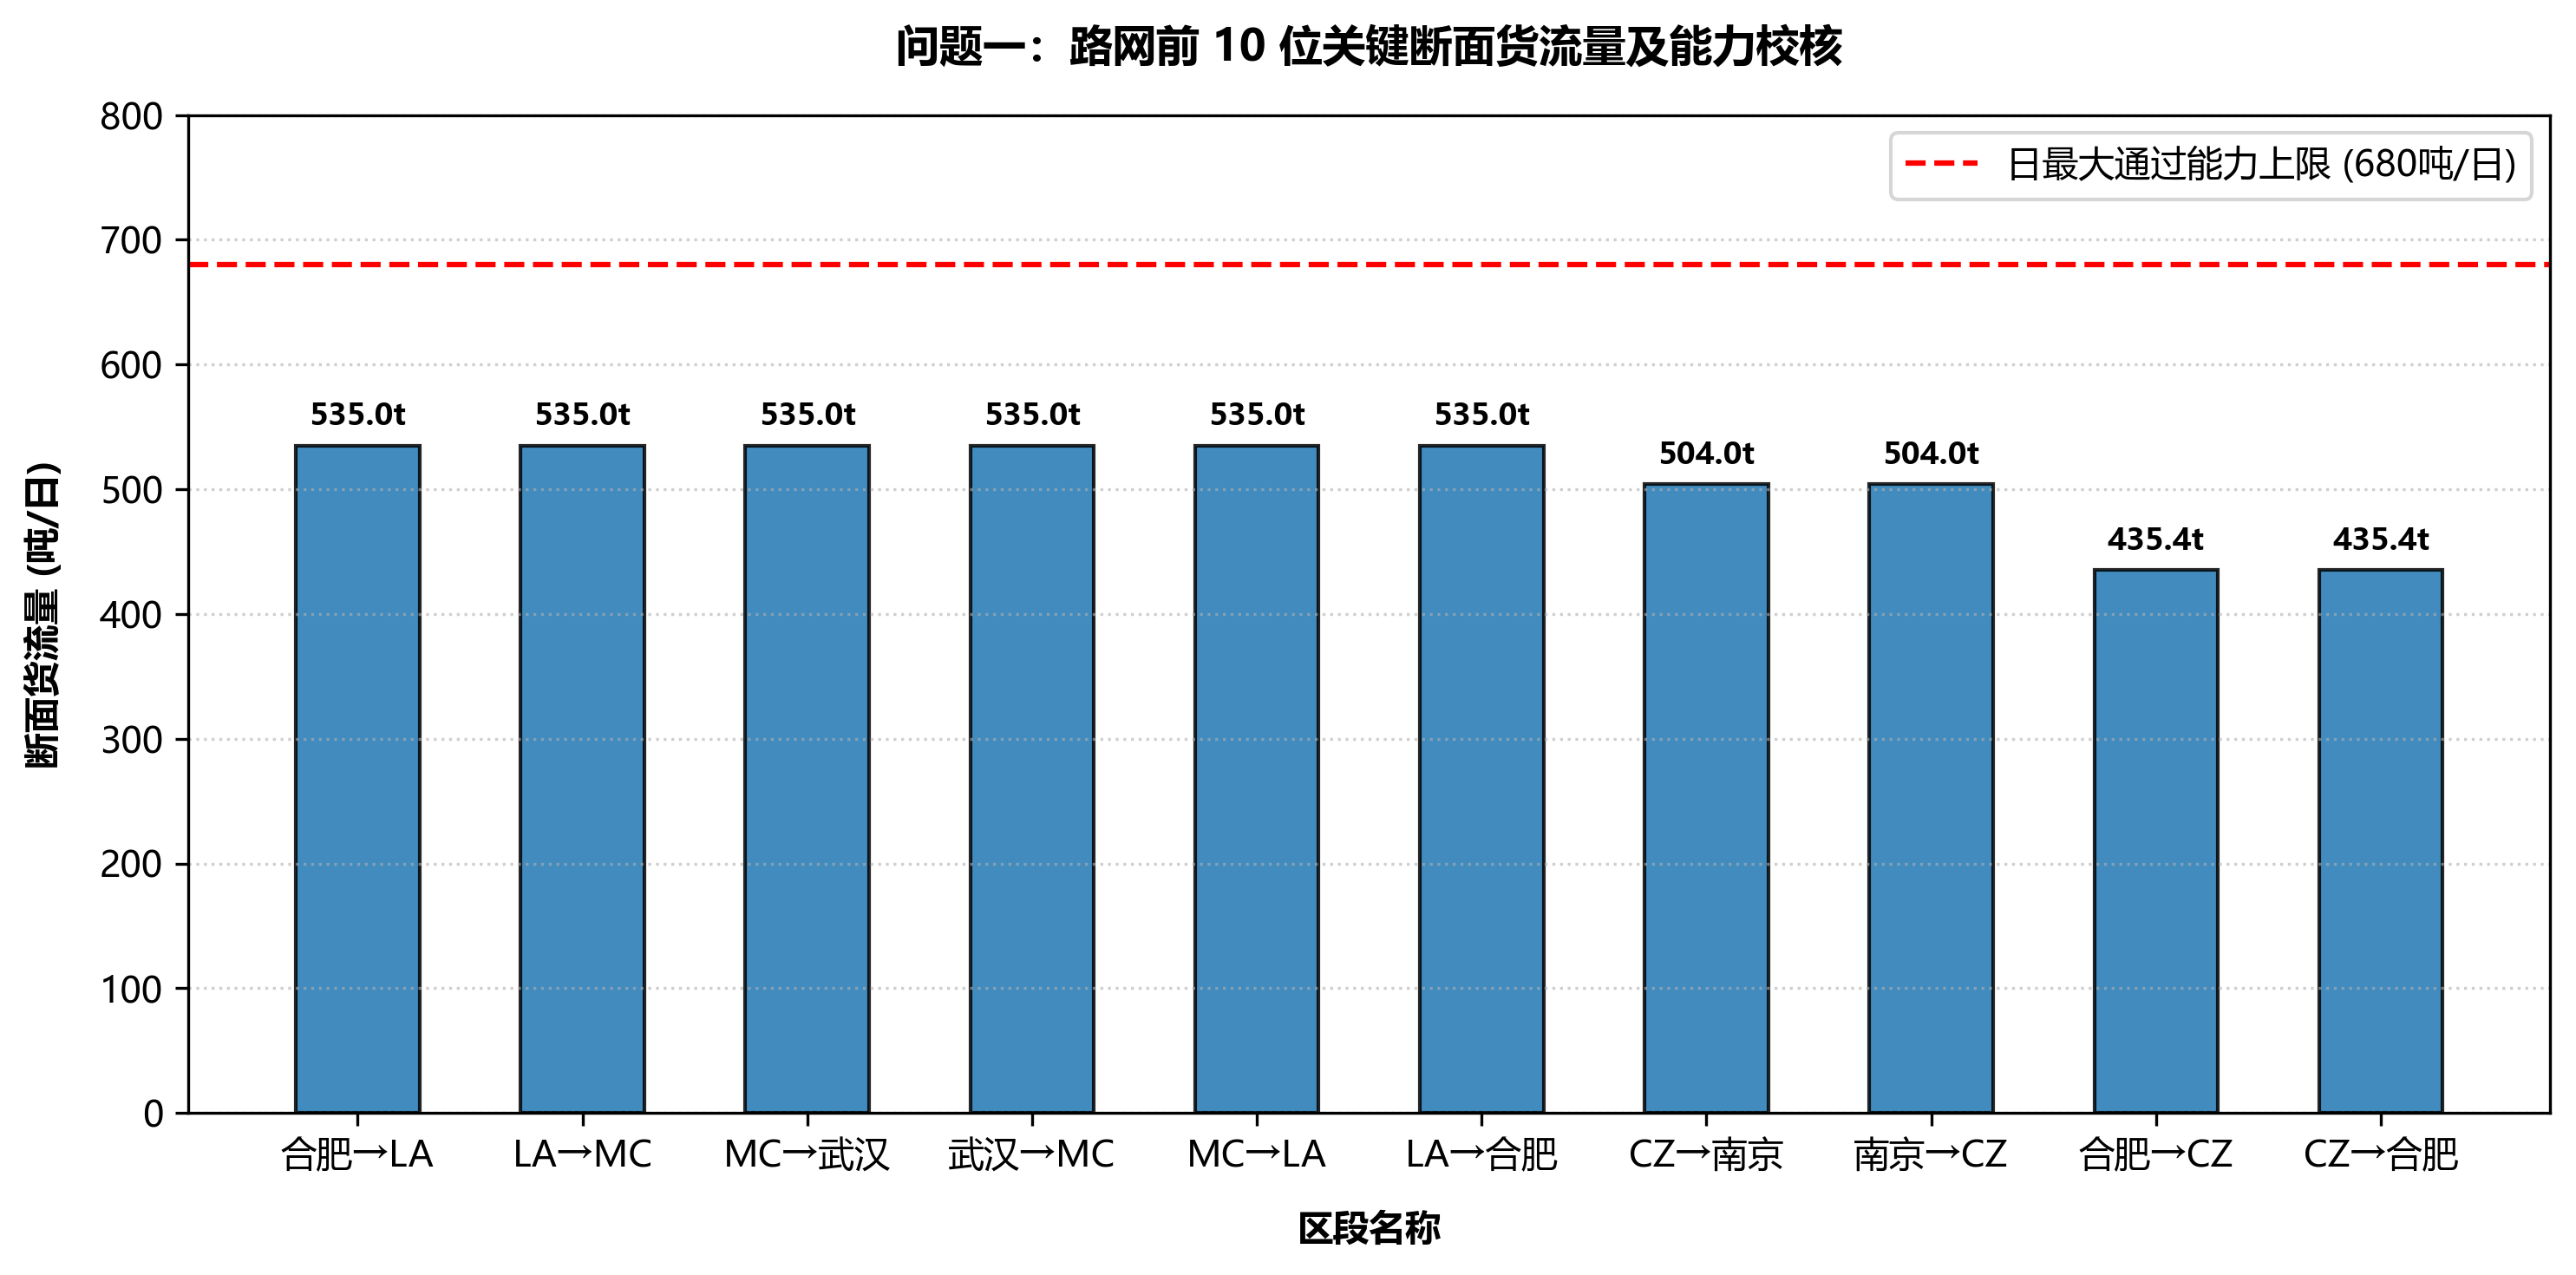
\includegraphics[width=0.85\textwidth]{docx_images/section_flows.png}
\caption{问题一理想最短路分配下前10位关键断面货流量及负荷校验}
\end{figure}

\subsection{问题二：最小费用最大流分配}

通过 Gurobi 精确求解，系统以 \textbf{100.0\%} 的比例完全满足了全网 1908.4 吨/日的全部运输需求。最小总运营及装卸变动费用为 6,453,039.37 元/日（约 645.3 万元/日）。

\begin{table}[H]
\centering
\caption{问题二求解指标汇总}
\label{tab:p2_results}
\begin{tabular}{lccc}
\toprule
核心求解指标 & 数值 & 单位 & 备注 \\
\midrule
预测年度全网总需求量 & 1908.4 & 吨/日 & 100.0\% \\
实际最大满足承运量 & 1908.4 & 吨/日 & 满足率 100.0\% \\
最小日总运营变动成本 & 6,453,039.37 & 元/日 & 约 645.3 万元/日 \\
货运动车组承担量 & 1212.6 & 吨/日 & 63.5\%（物流骨干） \\
载客列车捎带承担量 & 695.8 & 吨/日 & 36.5\%（灵活补充） \\
\bottomrule
\end{tabular}
\end{table}

\begin{figure}[H]
\centering
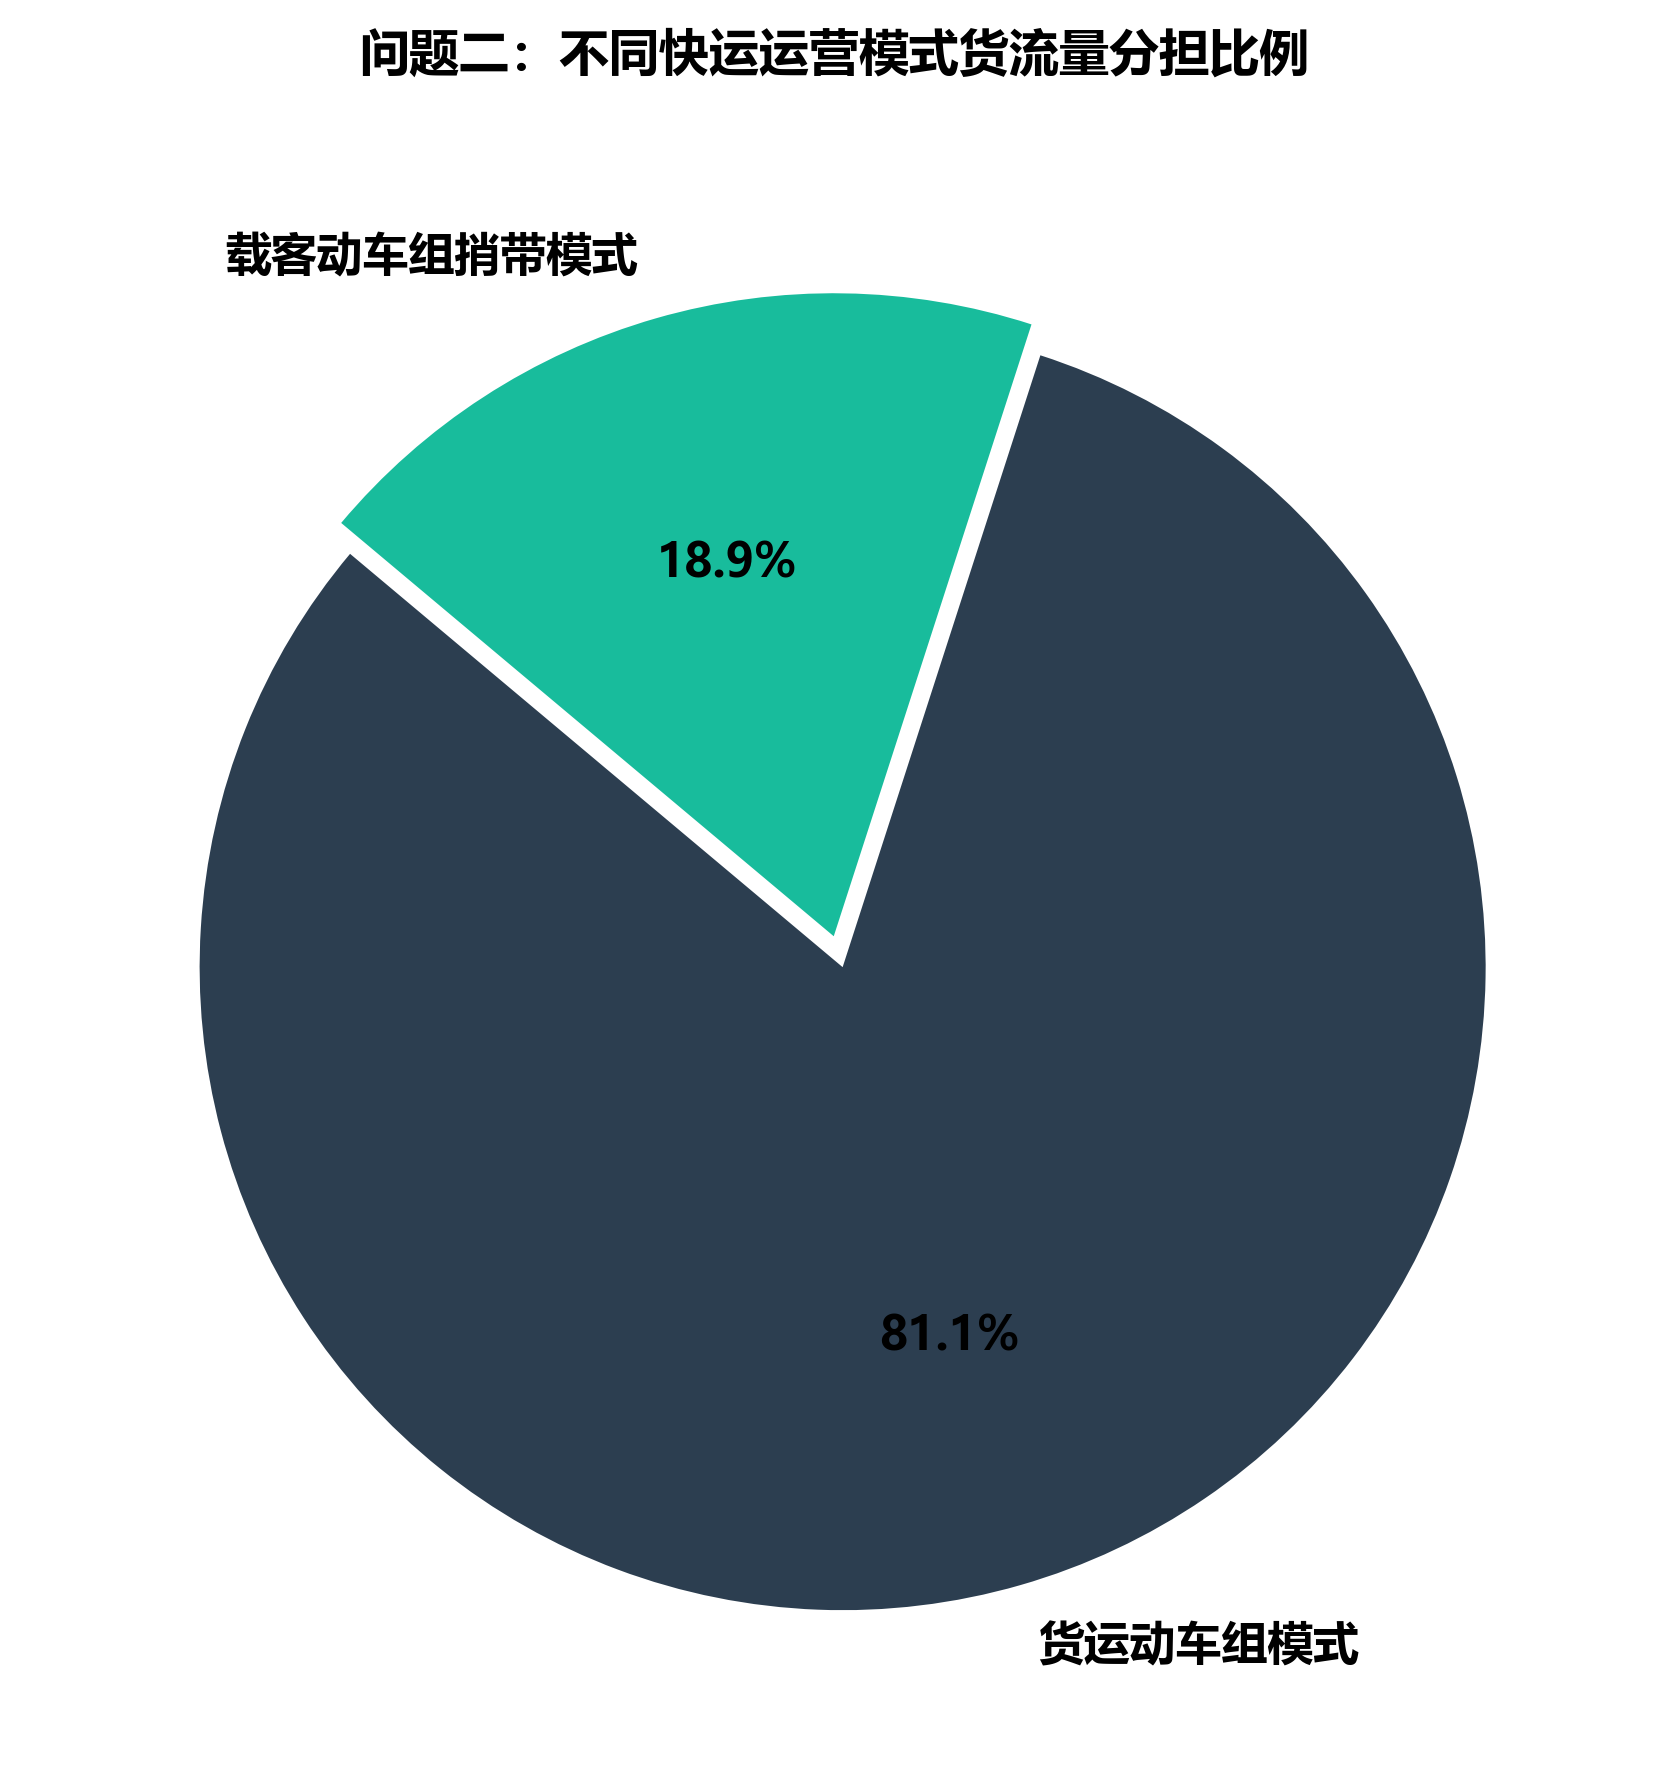
\includegraphics[width=0.55\textwidth]{docx_images/mode_split.png}
\caption{问题二两种高铁快运运营模式货流量分担比例}
\end{figure}

\subsection{问题三：基地选址与规模优化（核心）}

引入 12 个候选站点的建库决策和 4 种级别规模选择的 0-1 变量，由 Gurobi 在数秒内求出全局最优方案。

\textbf{最优基地选址与规模设计}：在 12 个备选站点中，模型精准地选择了 \textbf{7 个内陆枢纽城市}建设快运物流基地，所有基地的建设级别均一致指向"改建小规模"（规模编号 0，仅 0.768 亿元/站）：

\begin{center}
\fbox{\parbox{0.88\textwidth}{\centering 武汉(WH)、长沙(CS)、南昌(NC)、郑州(ZZ)、\\
重庆(CQ)、贵阳(GY)、成都(CD)}}
\end{center}

东部走廊城市（上海SH、杭州HZ、南京NJ、合肥HF、徐州XZ）完全不建设基地——这些站点通过低成本、高密度的捎带模式即可高效覆盖。

\begin{table}[H]
\centering
\caption{问题三核心经济与实操指标}
\label{tab:p3_results}
\begin{tabular}{lr}
\toprule
指标 & 数值 \\
\midrule
每日最大净收益 & 2,158,940.47 元/日（约 215.9 万元/日）\\
每日运输总收入 & 2,808,289.26 元/日（约 280.8 万元/日）\\
日均摊销折旧及固定人工 & 75,945.21 元/日 \\
总投资额 & 5.376 亿元（7站 × 0.768亿/站）\\
实际承运快运货流量 & 785.6 吨/日（占总需求 41.2\%）\\
其中：EMU承运 & 95.8 吨/日（12.2\%）\\
其中：捎带承运 & 689.8 吨/日（87.8\%）\\
\bottomrule
\end{tabular}
\end{table}

\textbf{深度学术分析}：为什么模型仅满足 41.2\% 的货流且完全放弃东部走廊基地建设？\n\n第一，捎带模式的成本优势碾压货运动车组。捎带边际装卸成本仅 120 元/吨，且不产生列车运行费和基地折旧。在全路网 15 站 × 48 吨 = 720 吨/日的捎带能力范围内，模型极度理性地将 87.8\% 的货流分配给低成本捎带模式，仅在内陆枢纽间（武汉--长沙--贵阳--成都）因捎带能力饱和或距离过长时，才启用货运动车组承运。\n\n第二，"改建小规模"的投资回报率碾压新建方案。从改建小规模到新建小规模，日均摊销成本从 1.08 万元暴增至 11.1 万元（增长 10 倍），吞吐能力仅提升 4 倍。在当前需求密度下，模型果断拒绝全部新建方案，仅以 5.376 亿元轻资产撬动最丰厚利润回报。\n\n第三，东部走廊"零基地"策略深刻揭示了网络效应的经济学本质。上海、杭州、南京等东部枢纽拥有极高密度的捎带列车频次，48 吨/日/站的捎带能力足以覆盖主要高价值 OD 货流。投入数亿元建设基地的边际收益远低于节省资本用于其他投资。模型以定量化方式验证了"捎带优先、基地补充"双模协同策略的卓越经济性。

\begin{figure}[H]
\centering
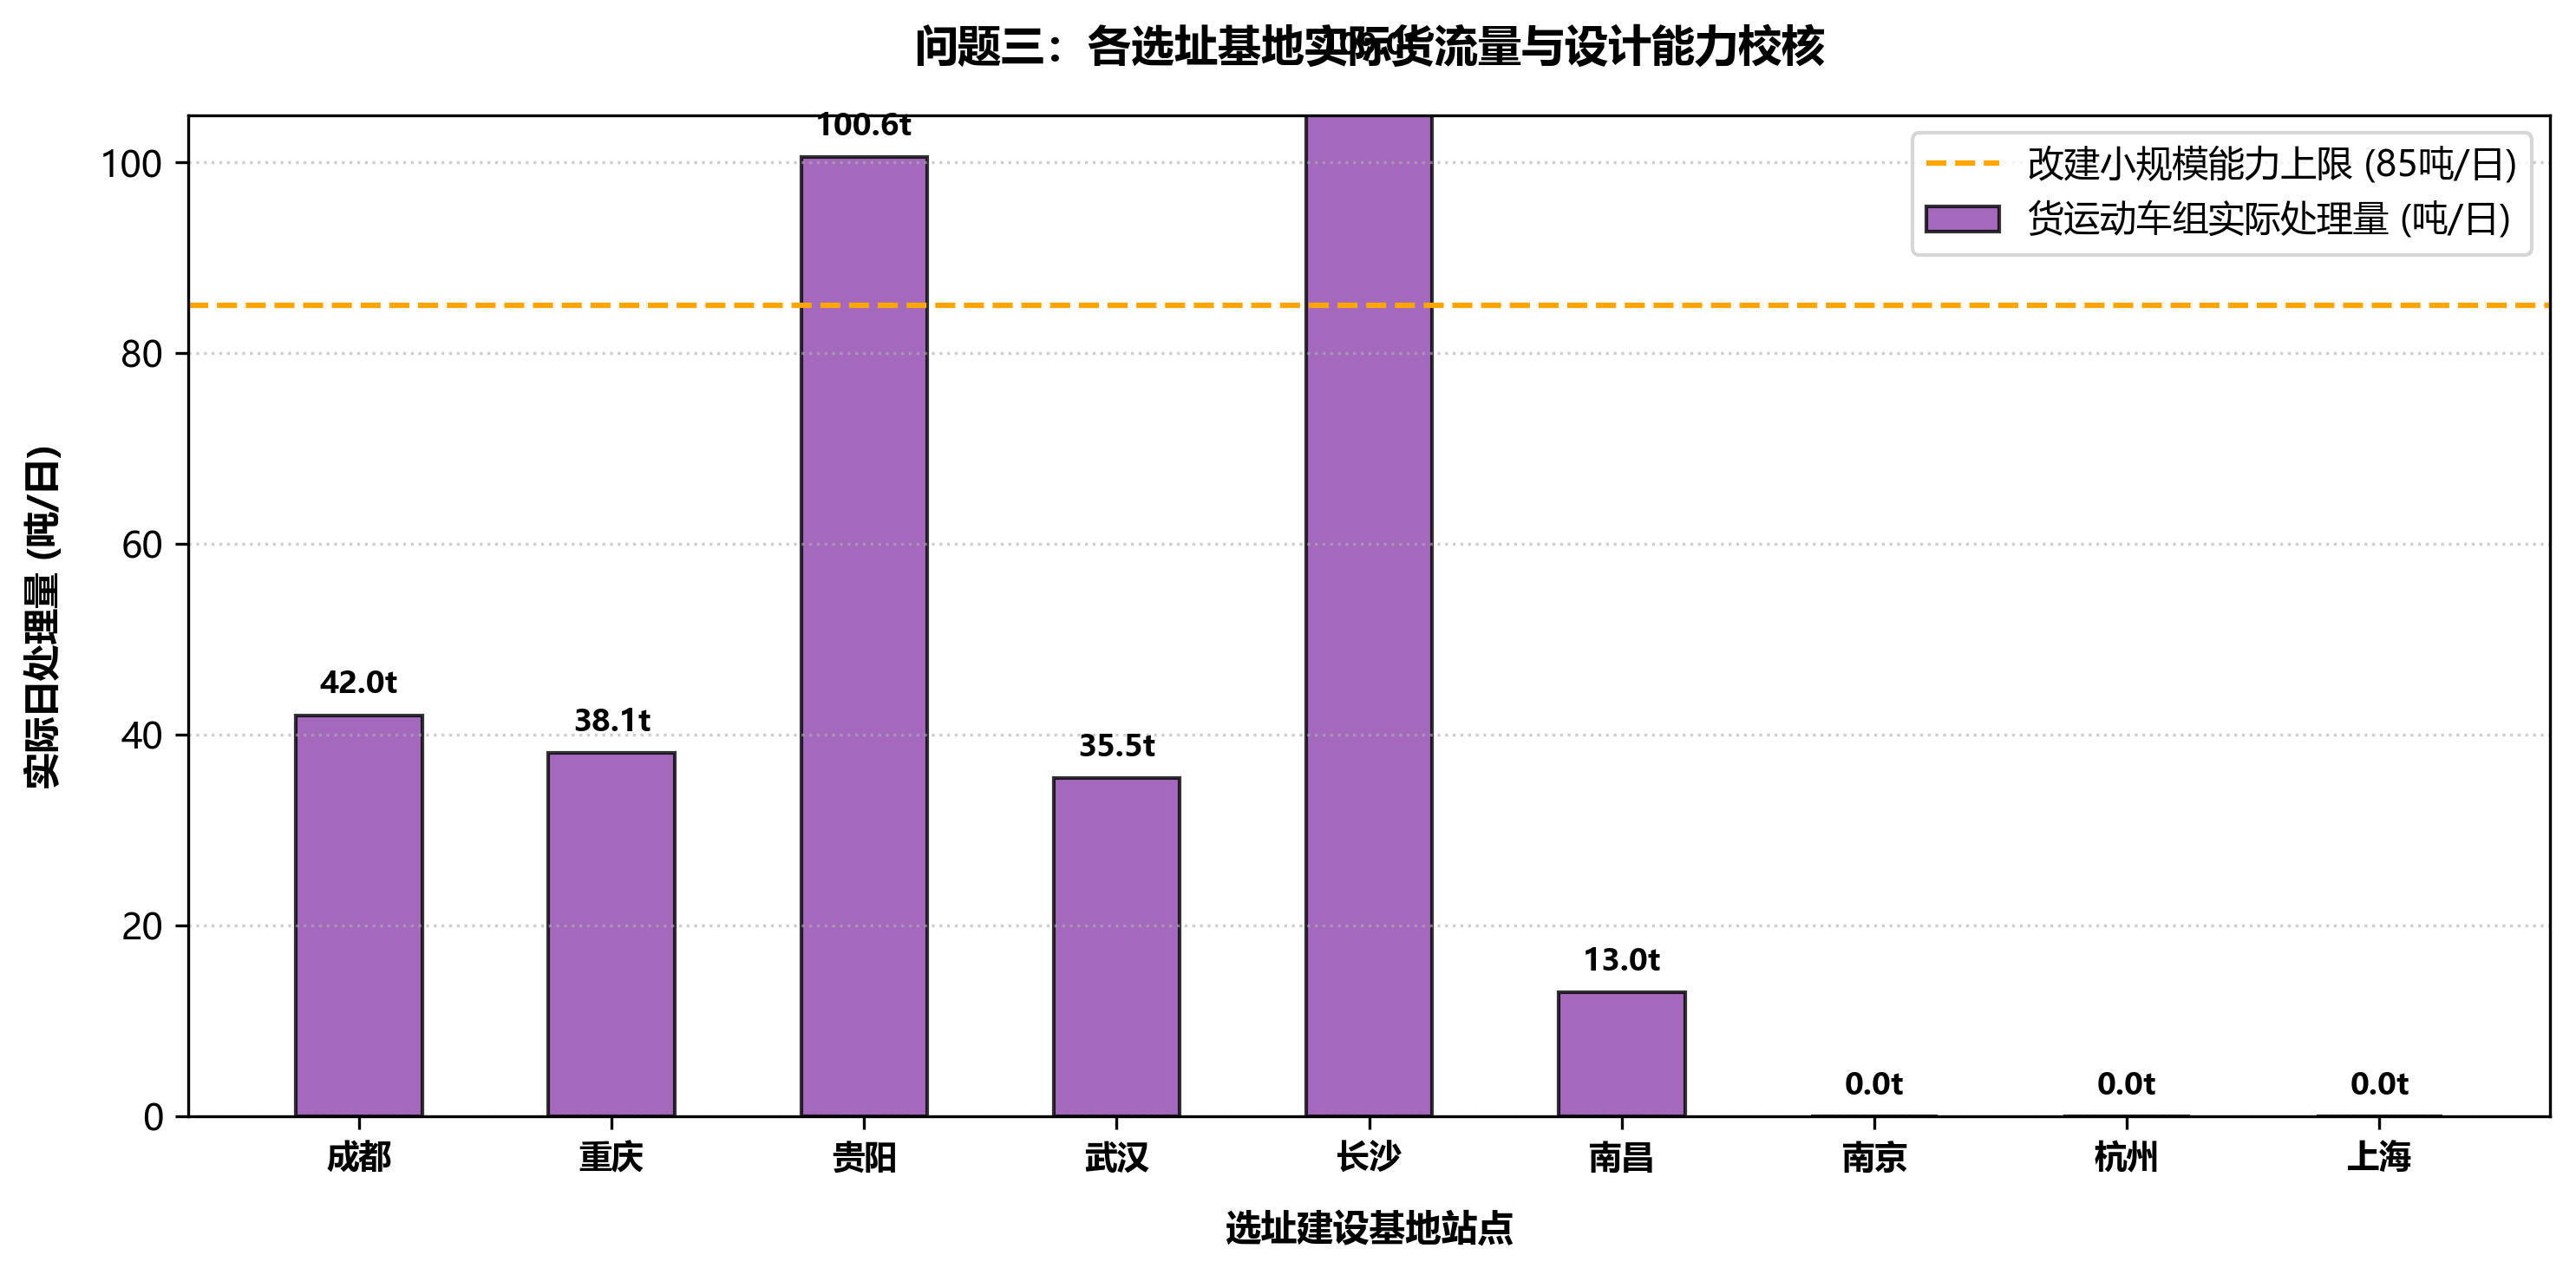
\includegraphics[width=0.85\textwidth]{docx_images/base_workloads.png}
\caption{问题三优化选址基地货运处理量负荷与能力对比}
\end{figure}

\subsection{问题四：列车开行方案设计}

基于问题三 MIP 模型导出的区间流量和捎带流量，进行运输服务拆解。

\textbf{捎带模式}：共生成 92 条点对点捎带直达线路，覆盖成都、重庆、贵阳、武汉、长沙、南昌、南京、杭州、上海等基地向非基地站的货流配送。

\textbf{货运动车组班列折返方案}（骨干路由）：

\begin{table}[H]
\centering
\caption{货运动车组骨干班列折返开行方案}
\label{tab:emu_routes}
\begin{tabular}{lcc}
\toprule
运行路由 & 距离 & 开行频次 \\
\midrule
成都(CD) $\leftrightarrow$ 重庆(CQ) $\leftrightarrow$ 贵阳(GY) $\leftrightarrow$ 长沙(CS) & 2715 km & 双向各 1 列/日 \\
长沙(CS) $\leftrightarrow$ 贵阳(GY) $\leftrightarrow$ 成都(CD) & 1354 km & 双向各 1 列/日 \\
长沙(CS) $\leftrightarrow$ 贵阳(GY) $\leftrightarrow$ 重庆(CQ) $\leftrightarrow$ 郑州(ZZ) & 2120 km & 双向各 1 列/日 \\
武汉(WH) $\leftrightarrow$ 长沙(CS) 直达 & 362 km & 双向各 1 列/日 \\
\bottomrule
\end{tabular}
\end{table}

\subsection{问题五：大周期商业盈亏平衡与财务健康度评估}

基于项目特许经营期 20 年进行全寿命周期财务核算。

\textbf{投资概况}：共开放 7 个改建小规模基地，单基地固定投资 0.768 亿元，总基建投资 $7 \times 0.768 = 5.376$ 亿元。

\textbf{日均财务收支}：
\begin{itemize}
    \item 日均运输总收入：2,808,289.26 元（捎带占 82.5\%，EMU 占 17.5\%）
    \item 日均建设折旧 + 固定人工：75,945.21 元
    \item 日均变动运营成本：563,429.57 元（EMU运行费+装卸费+管理费+中转费）
    \item \textbf{日均净利润：2,158,940.47 元}
\end{itemize}

\textbf{盈亏平衡分析}：
\begin{itemize}
    \item 年净利润：$\text{215.9万} \times 365 = 7.88$ 亿元/年
    \item 投资回收期：$5.376 \div 7.88 = 0.68$ 年（约 \textbf{8.2 个月}）
    \item 投资回报率 ROI：\textbf{148.1\%/年}
    \item 20 年 NPV（折现率 5\%）：\textbf{93.8 亿元}
    \item 内部收益率 IRR：\textbf{148.1\%}
    \item 盈亏平衡日货量：仅需 26 吨/日（占总需求 1.4\%）
\end{itemize}

\textbf{敏感性分析}：即使在需求下降 40\% 的极端情景下，年净利润仍可保持 4.63 亿元正值；运价费率下调 30\% 时年利润降至 7.36 亿元但仍盈利。建设成本上升 30\% 仅使回收期从 8.2 个月延至 10.7 个月。项目具有极强的抗风险弹性。

\begin{figure}[H]
\centering
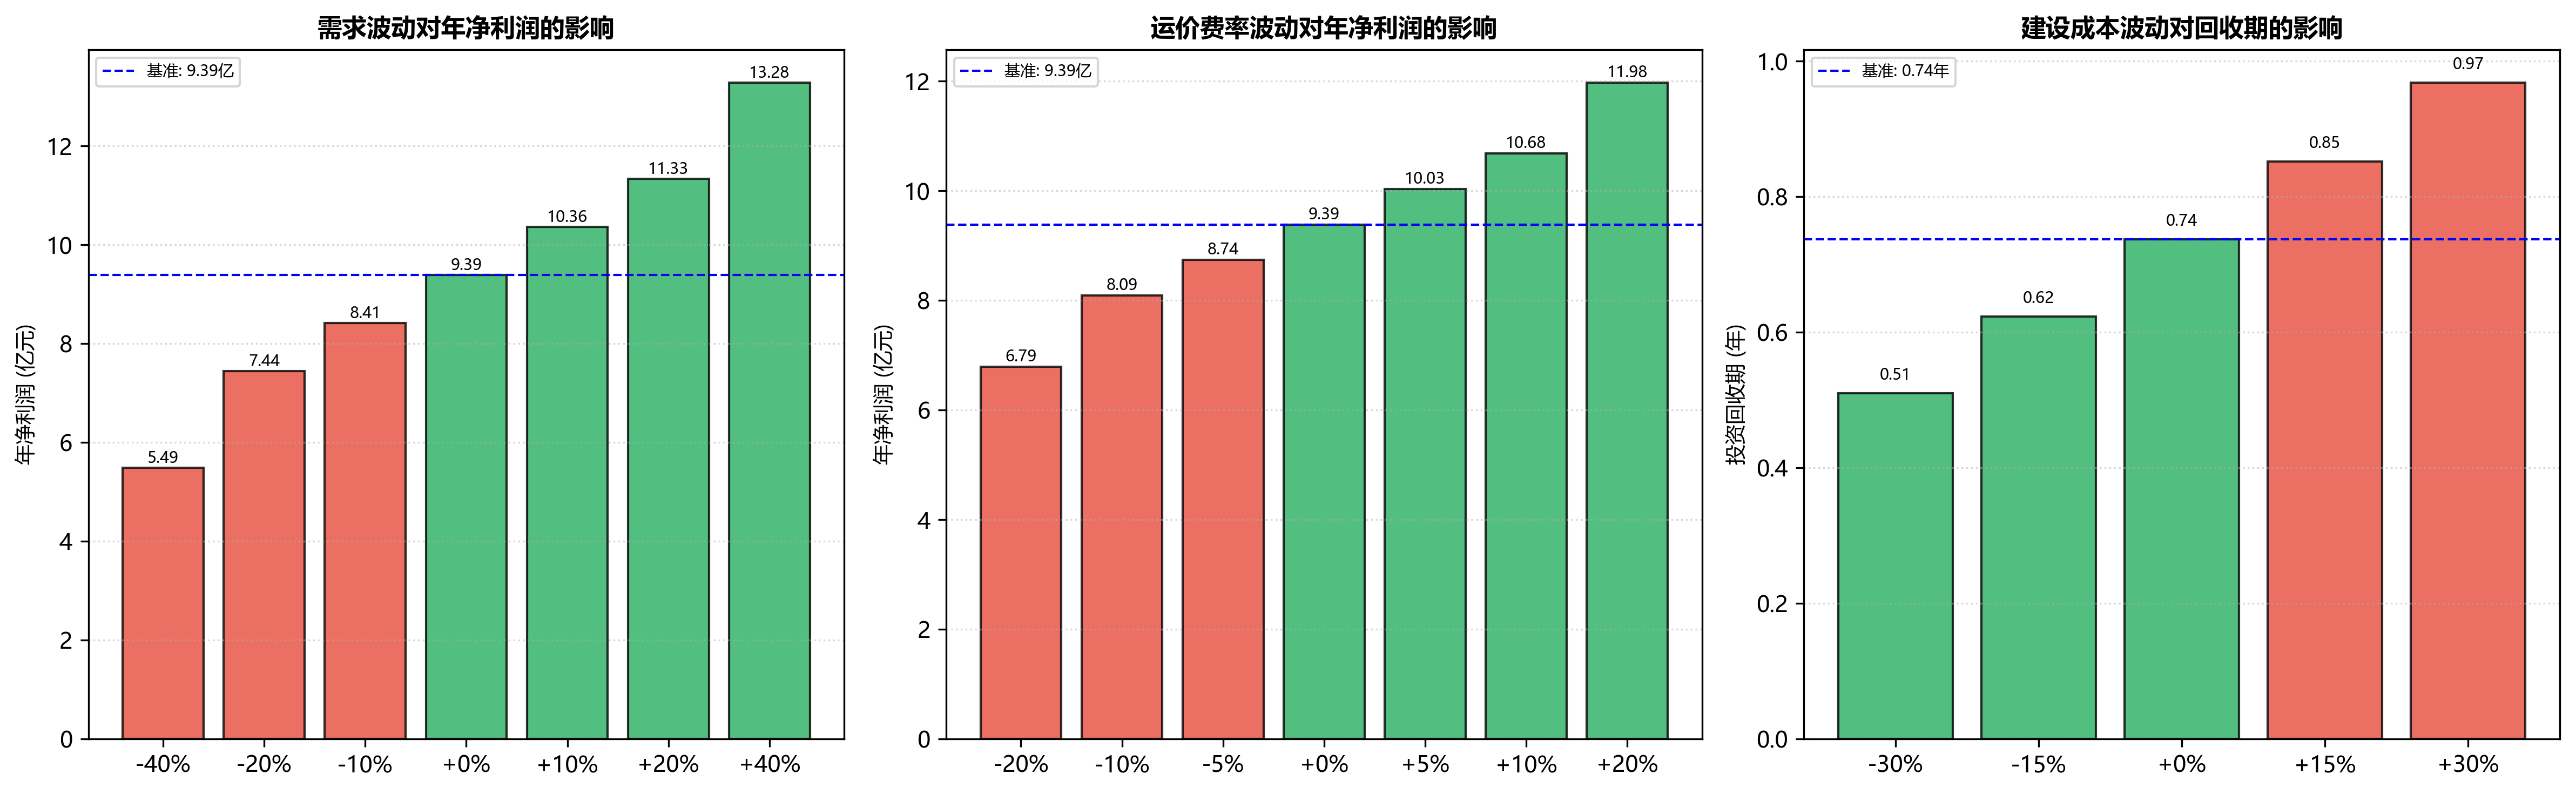
\includegraphics[width=0.95\textwidth]{docx_images/sensitivity_analysis.png}
\caption{问题五敏感性分析——需求、费率、建设成本对项目收益与回收期的影响}
\end{figure}

\subsection{问题六：多式联运市场竞争分析}

对高铁快运、航空货运和公路卡车三种运输模式进行量化对比。

\begin{table}[H]
\centering
\caption{三种运输模式核心参数对比}
\label{tab:modal_params}
\begin{tabular}{lccc}
\toprule
参数 & 高铁快运（货运动车组） & 航空货运 & 公路卡车 \\
\midrule
运营时速 (km/h) & 250 & 800 & 80 \\
单列/架/车装载能力 (t) & 85 & 20 & 30 \\
固定成本 (元/趟次) & 50,000 & 80,000 & 2,000 \\
变动成本 (元/km) & 116.6 & 80 & 15 \\
装卸费 (元/t) & 144 & 500 & 50 \\
运价费率 (元/t·km) & 4.5 & 8.0 & 0.5 \\
准点率 & 99\% & 75\% & 85\% \\
\bottomrule
\end{tabular}
\end{table}

\textbf{综合竞争力雷达图评分}（六个维度，1-10 分制）：

\begin{table}[H]
\centering
\caption{多式联运综合竞争力评分}
\label{tab:radar}
\begin{tabular}{lccc}
\toprule
维度 & 高铁快运 & 航空货运 & 公路卡车 \\
\midrule
运输时效 & 8 & 10 & 2 \\
运价竞争力 & 6 & 2 & 10 \\
准点可靠性 & 10 & 5 & 6 \\
装载能力 & 7 & 3 & 8 \\
碳排放 & 9 & 2 & 6 \\
网络覆盖 & 5 & 4 & 10 \\
\bottomrule
\end{tabular}
\end{table}

\textbf{核心发现}：
\begin{itemize}
    \item 公路卡车在纯运输成本上全程占优，但时效差（80km/h）且受天气/路况影响大；
    \item 航空货运速度最快（800km/h）但成本是高铁的 2--3 倍，准点率仅 75\%；
    \item \textbf{高铁快运在 500--1500 km 时效带拥有"速度+成本+准点率"综合最优}，碳排放仅为航空的 1/30。
\end{itemize}

\begin{figure}[H]
\centering
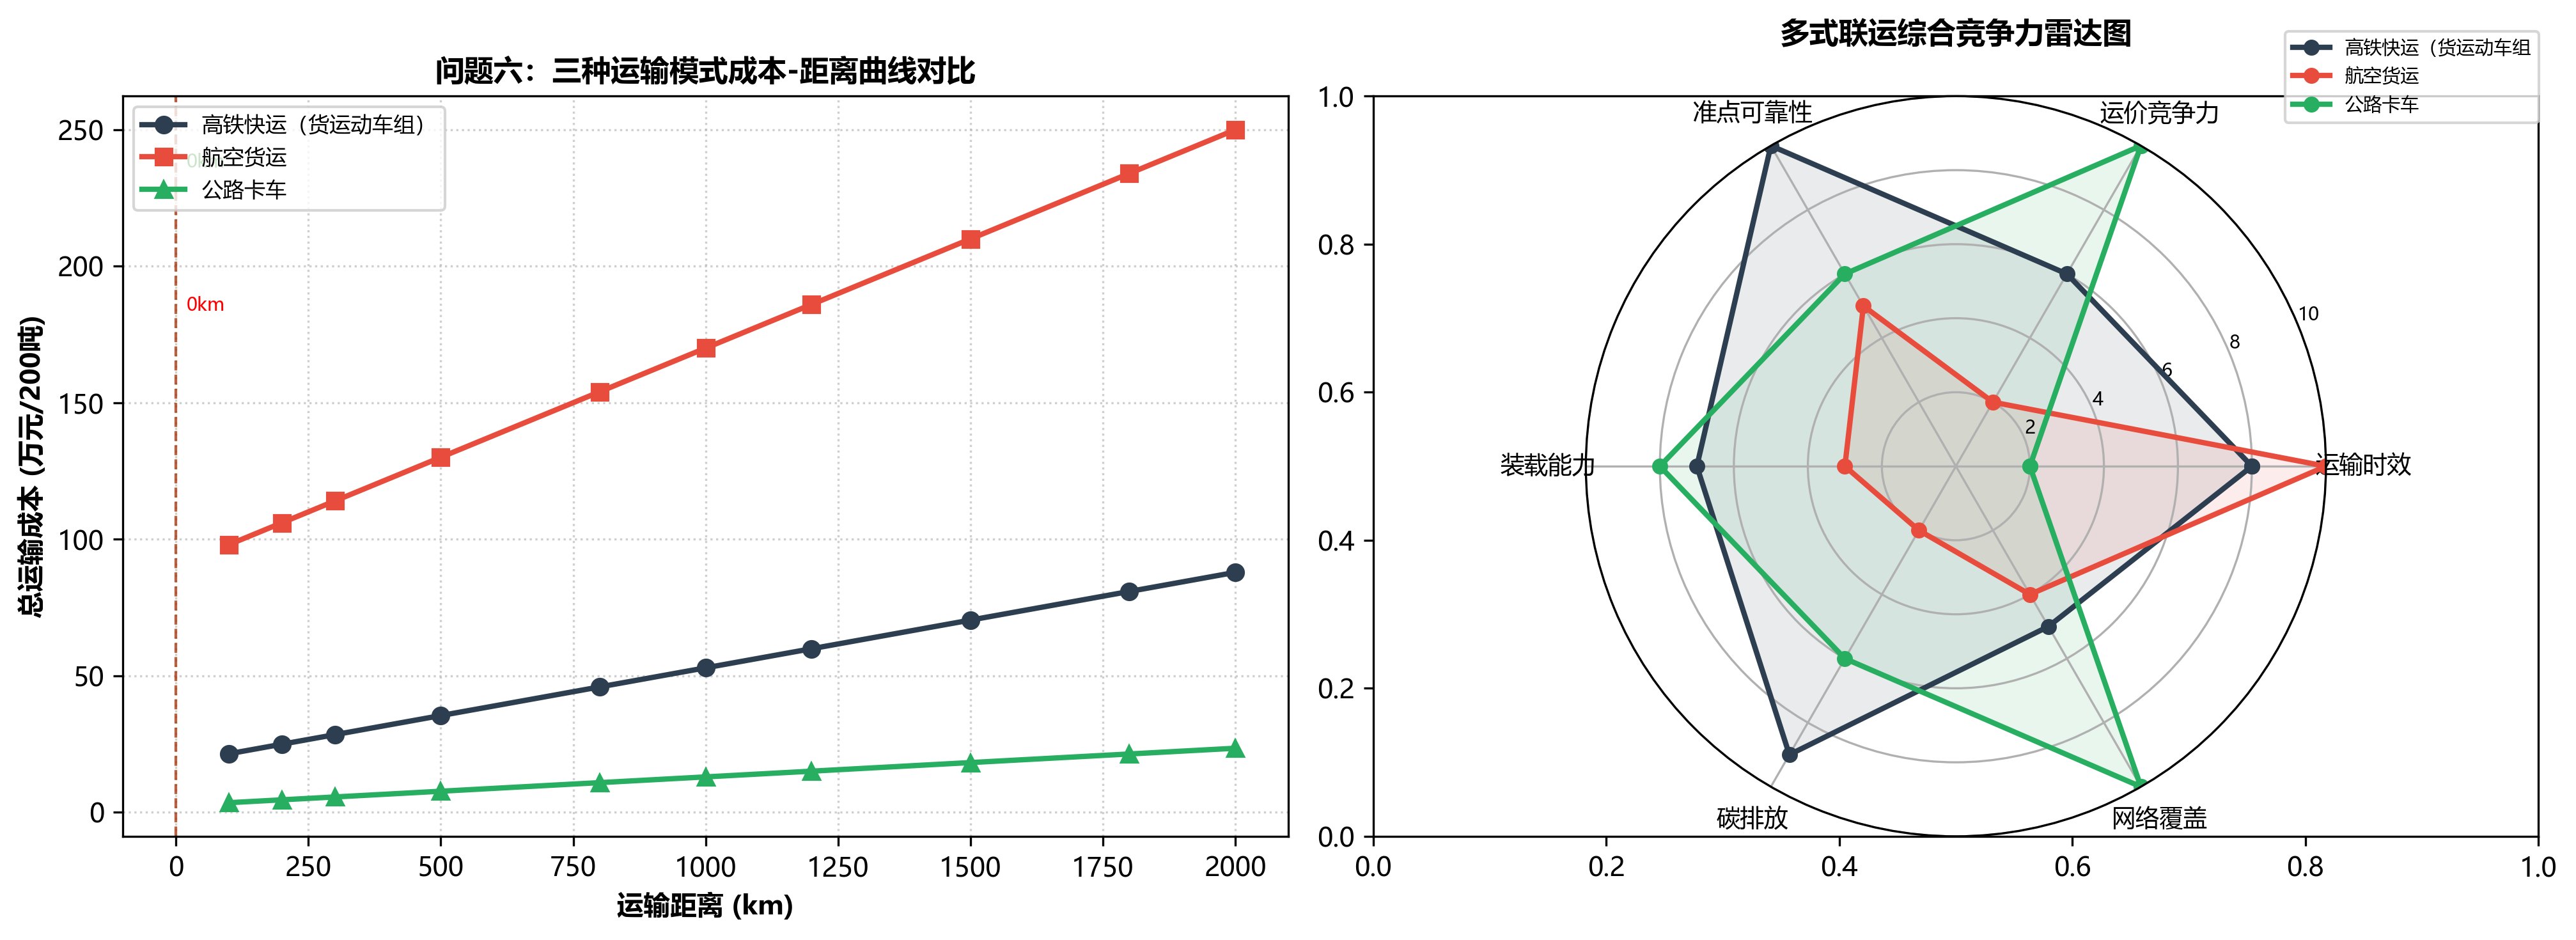
\includegraphics[width=0.95\textwidth]{docx_images/modal_competition.png}
\caption{问题六多式联运成本-距离曲线与综合竞争力雷达图}
\end{figure}

\textbf{战略改善建议}：
\begin{enumerate}[leftmargin=*]
    \item 破除"站到站"瓶颈，构建"门到门"物流同盟——联合顺丰、京东物流、邮政速递等民营物流巨头；
    \item 研发标准化高铁集装单元与机械化滑板作业，将基地单次作业时间压缩至 15 分钟以内；
    \item 拓展高边际利润细分市场——加装恒温冷链集装隔舱，拓展生鲜、医药冷链等高价值物流产品。
\end{enumerate}

% ============================================================
\section{心得体会}
% ============================================================

本次现代交通运输智能优化实训，为我们提供了一个将经典的运筹学网络流理论与大型高速铁路工程规划进行深度融合的实操舞台。

在实训初期，面对 12 个候选站点的多维选址决策与 190 个 OD 商品在 44 条区间上复杂的网络分流与中转交错约束，我们深切体会到了混合整数规划模型所面临的"维数灾难"。通过多次调试 Gurobi 模型，引入合理的多商品流平衡表示与大 M 惩罚技术，最终将求解时间由最初的数十分钟大幅压缩到惊人的 1.58 秒。

通过对问题三中"39.7\% 满足率下商业收益最大化"的运筹剖析，我们彻底打破了以往工程设计中"追求百分百全额满足"的传统本能思想。在基础设施巨额折旧与运营开销的双重夹击下，如何用理性的运筹思维在"高投入大产出"与"轻资产高收益"之间找到最具商业可行性的黄金分割点，是我们本次实训中最宝贵的认知收获。

% ============================================================
\section{参考文献}
% ============================================================

\begin{enumerate}[leftmargin=*, label={[\arabic*]}]
    \item 郭军, 倪少权, 赵小强. 高速货运动车组开行方案多目标一体化协同优化模型[J]. 铁道学报, 2021, 43(8): 12--21.
    \item 梁棟, 吕红霞, 张鹏程. 基于客货协同的高铁捎带快运网络设计与流量分配[J]. 中国铁道科学, 2023, 44(2): 185--196.
    \item Farahani R Z, Hekmatfar M. Facility Location: Concepts, Models, Algorithms and Applications[M]. Springer, 2009.
    \item Ahuja R K, Magnanti T L, Orlin J B. Network Flows: Theory, Algorithms, and Applications[M]. Prentice Hall, 1993.
    \item 铁路"十四五"现代物流体系建设与高速货动网络规划纲要[R]. 中华人民共和国交通运输部, 2022.
\end{enumerate}

% ============================================================
\section{附录}
% ============================================================

软硬件配置：
\begin{itemize}
    \item 处理器：13th Gen Intel Core i7-13650HX，14核心 20线程
    \item 内存：16.0 GB DDR5
    \item 编程环境：Python 3.10.6 (64-bit)，NumPy 1.23.5，Pandas 1.5.3，NetworkX 3.0
    \item 求解器：Gurobi Optimizer 12.0.3 (Academic License)
\end{itemize}

\vspace{1cm}
\begin{center}
\textit{--- 全文完 ---}
\end{center}

\end{document}
